\section{傅里叶级数}

\subsection{傅里叶级数的三角式}

\begin{BoxDefinition}[三角函数集]
    三角函数集
    \begin{Equation}
        \left\{1,\cos(n\Omega t),\sin(n\Omega t), n=1,2,\dots\right\}
    \end{Equation}
    在一个周期内是一个完备的正交函数集。

    由积分可知
    \begin{Equation}
        \int_{-\frac{T}{2}}^{\frac{T}{2}}\cos(n\Omega t )\cdot\sin(m\Omega t)dt = 0
    \end{Equation}
    \begin{Equation}
        \int_{-\frac{T}{2}}^{\frac{T}{2}}\cos(n\Omega t )\cdot\cos(m\Omega t)dt = \left\{
        \begin{aligned}
            \frac{T}{2} & , & m=n     \\
            0           & , & m\neq n
        \end{aligned}
        \right.
    \end{Equation}
    \begin{Equation}
        \int_{-\frac{T}{2}}^{\frac{T}{2}}\sin(n\Omega t )\cdot\sin(m\Omega t)dt = \left\{
        \begin{aligned}
            \frac{T}{2} & , & m=n     \\
            0           & , & m\neq n
        \end{aligned}
        \right.
    \end{Equation}
\end{BoxDefinition}

\begin{BoxDefinition}[傅里叶级数的三角函数形式]
    设$f(t) = f(t+mT)$,即$f(t)$为周期信号,且$\Omega = \frac{2\pi}{T}$,满足狄里赫利(Dirichlet)条件,可分解为以下三角级数,称为傅里叶级数。
    \begin{Equation}
        f(t) = \frac{a_0}{2} + \sum\limits_{n=1}^{\infty}a_n\cos(n\Omega t)+ \sum\limits_{n=1}^{\infty}b_n \sin(n\Omega t)
    \end{Equation}
    其中系数$a_n$和$b_n$称为傅里叶系数,满足
    \begin{Equation}
        a_n = \frac{2}{T}  \int_{-\frac{T}{2}}^{\frac{T}{2}}f(t)\cos(n\Omega t)dt
    \end{Equation}
    \begin{Equation}
        b_n = \frac{2}{T}  \int_{-\frac{T}{2}}^{\frac{T}{2}}f(t)\sin(n\Omega t)dt
    \end{Equation}
    且$a_n$是$n$的偶函数,$b_n$是$n$的奇函数。

    合并同频率项
    \begin{Equation}
        f(t) = \frac{A_0}{2} + \sum\limits_{n=1}^{\infty}A_n\cos(n\Omega t + \varphi_n)
    \end{Equation}
    其中
    \begin{Equation}
        \begin{array}{ll}
            A_0 = a_0                  \\
            A_n = \sqrt{a_n^2 + b_n^2} \\
            \varphi_n = - \arctan\frac{b_n}{a_n}
        \end{array}
    \end{Equation}
    可见$A_n$是$n$的偶函数,$\varphi_n$是$n$的奇函数。

    且有
    \begin{Equation}
        a_n = A_n\cos\varphi_n,\ b_n = -A_n\sin\varphi_n,\ n = 1,2,\dots
    \end{Equation}
    合并同频率项式中的$\frac{A_0}{2}$称为直流分量,$A_1\cos(\Omega t + \varphi_1)$称为基波或一次谐波,

    $A_n\cos(n\Omega t + \varphi_n)$称为$n$次谐波。
\end{BoxDefinition}

\subsection{波形的对称性与谐波特性}

\begin{BoxProperty}[波形的对称性]
    波形为偶函数时满足
    \begin{Equation}
        f(t)=f(-t)
    \end{Equation}
    此时$b_n=0$,展开为余弦级数。

    波形为奇函数时满足
    \begin{Equation}
        f(t)=-f(-t)
    \end{Equation}
    此时$a_n=0$,展开为正弦级数。
\end{BoxProperty}

\begin{BoxProperty}[波形的谐波特性]
    \begin{Figure}[奇谐函数]
        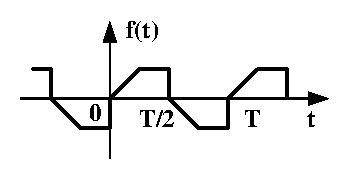
\includegraphics[width=40mm]{visio/4.1.pdf}
    \end{Figure}
    $f(t)$为奇谐函数$f(t)=-f(t\pm \frac{T}{2})$时,傅里叶级数满足
    \begin{Equation}
        a_0=a_2=\dots=b_2=b_4=0
    \end{Equation}
    即只含奇次谐波分量,不含偶次谐波分量。
    \begin{Figure}[偶谐函数]
        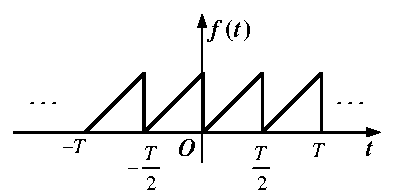
\includegraphics[width=40mm]{visio/4.2.pdf}
    \end{Figure}
    $f(t)$为偶谐函数$f(t)=f(t\pm \frac{T}{2})$时,傅里叶级数满足
    \begin{Equation}
        a_1=a_3=\dots=b_1=b_3=0
    \end{Equation}
    即只含偶次谐波分量,不含奇次谐波分量。
\end{BoxProperty}

\subsection{傅里叶级数的指数形式}

\begin{BoxDefinition}[傅里叶级数的指数形式]
    虚指数函数集
    \begin{Equation}
        \left\{e^{jn\Omega t},n=0,\pm 1,\pm 2, \dots\right\}
    \end{Equation}
    傅里叶级数的指数形式
    \begin{Equation}
        f(t) = \sum\limits_{n=-\infty}^{\infty}F_n e^{jn\Omega t}
    \end{Equation}
    傅里叶系数
    \begin{Equation}
        F_n = \frac{1}{T}\int_{-\infty}^{\infty}f(t)e^{-jn\Omega t}dt
    \end{Equation}
    由欧拉公式
    \begin{Equation}
        e^{i\theta} = \cos \theta + i sin \theta
    \end{Equation}
    可推导出
    \begin{Equation}
        \cos x = \frac{e^{\mathrm{j}x}+e^{-\mathrm{j}x}}{2}
    \end{Equation}
    \begin{Equation}
        \sin x = \frac{e^{\mathrm{j}x}-e^{-\mathrm{j}x}}{2\mathrm{j}}
    \end{Equation}
    则三角函数形式的傅里叶级数可推导为
    \begin{Equation}
        \begin{aligned}
            f(t) & = \frac{A_0}{2}+\sum\limits_{n=1}^{\infty} A_n \cos(n\Omega t +\varphi_n)                                                                                                                       \\
                 & = \frac{A_0}{2}+\sum\limits_{n=1}^{\infty} \frac{A_n}{2}\left[e^{\mathrm{j}(n\Omega t+\varphi_n)}+e^{-\mathrm{j}(n\Omega t+\varphi_n)}\right]                                                   \\
                 & = \frac{A_0}{2}+\frac{1}{2}\sum\limits_{n=1}^{\infty}A_ne^{\mathrm{j}\varphi_n}e^{\mathrm{j}n\Omega t}+\frac{1}{2}\sum\limits_{n=1}^{\infty}A_ne^{-\mathrm{j}\varphi_n}e^{-\mathrm{j}n\Omega t}
        \end{aligned}
    \end{Equation}
    令$A_{-n}=A_n,\varphi_{-n}=\varphi_n,A_0=A_0e^{\mathrm{j}\varphi_0}e^{\mathrm{j}0\Omega t},\varphi_0=0$,则
    \begin{Equation}
        \begin{aligned}
            f(t) & = \frac{A_0}{2}+\frac{1}{2}\sum\limits_{n=1}^{\infty}A_ne^{\mathrm{j}\varphi_n}e^{\mathrm{j}n\Omega t}+\frac{1}{2}\sum\limits_{n=-1}^{-\infty}A_ne^{\mathrm{j}\varphi_n}e^{\mathrm{j}n\Omega t} \\
                 & = \frac{1}{2}\sum\limits_{n=-\infty}^{\infty}A_ne^{\mathrm{j}\varphi_n}e^{\mathrm{j}n\Omega t}
        \end{aligned}
    \end{Equation}
\end{BoxDefinition}

\begin{BoxProperty}[傅里叶系数之间的关系]
    傅里叶系数之间满足以下关系
    \begin{Equation}
        F_n = \frac{1}{2}A_ne^{\mathrm{j}\varphi_n} = |F_n|e^{\mathrm{j}\varphi_n} = \frac{1}{2}(a_n-\mathrm{j}b_n)
    \end{Equation}
    \begin{Equation}
        F_0 = \frac{A_0}{2}
    \end{Equation}
    \begin{Equation}
        |F_0| = \frac{1}{2}\sqrt{a_n^2+b_n^2} = \frac{1}{2}A_n
    \end{Equation}
    \begin{Equation}
        \varphi_n = \arctan(-\frac{b_n}{a_n})
    \end{Equation}
    \begin{Equation}
        a_n = A_n\cos\varphi_n
    \end{Equation}
    \begin{Equation}
        b_n = -A_n\sin\varphi_n
    \end{Equation}
    其中$n$的奇函数有:$a_n,A_n,|F_n|$

    $n$的偶函数有:$b_n,\varphi_n$
\end{BoxProperty}


\subsection{周期信号的功率}

\begin{BoxFormula}[Parseval等式]
    周期信号一般为功率信号,其平均功率为
    \begin{Equation}
        P = \frac{1}{T}\int_{0}^{T}f^2(t)dt=\left(\frac{A_0}{2}\right)^2+\sum\limits_{n=1}^{\infty}\frac{1}{2}A_n^2=\sum\limits_{n=-\infty}^{\infty}|F_n|^2
    \end{Equation}
    其中$\left(\frac{A_0}{2}\right)^2$为直流功率,$\sum\limits_{n=1}^{\infty}\frac{1}{2}A_n^2$为各次谐波功率和。
\end{BoxFormula}
